\documentclass[border=5mm]{standalone}

\usepackage{tikz}
\usetikzlibrary{arrows.meta, angles, quotes}

\definecolor{darkblue}{rgb}{0.1, 0.2, 0.6}
\definecolor{darkgreen}{rgb}{0.1, 0.5, 0.1}
\definecolor{darkred}{rgb}{0.6, 0.1, 0.1}

\begin{document}
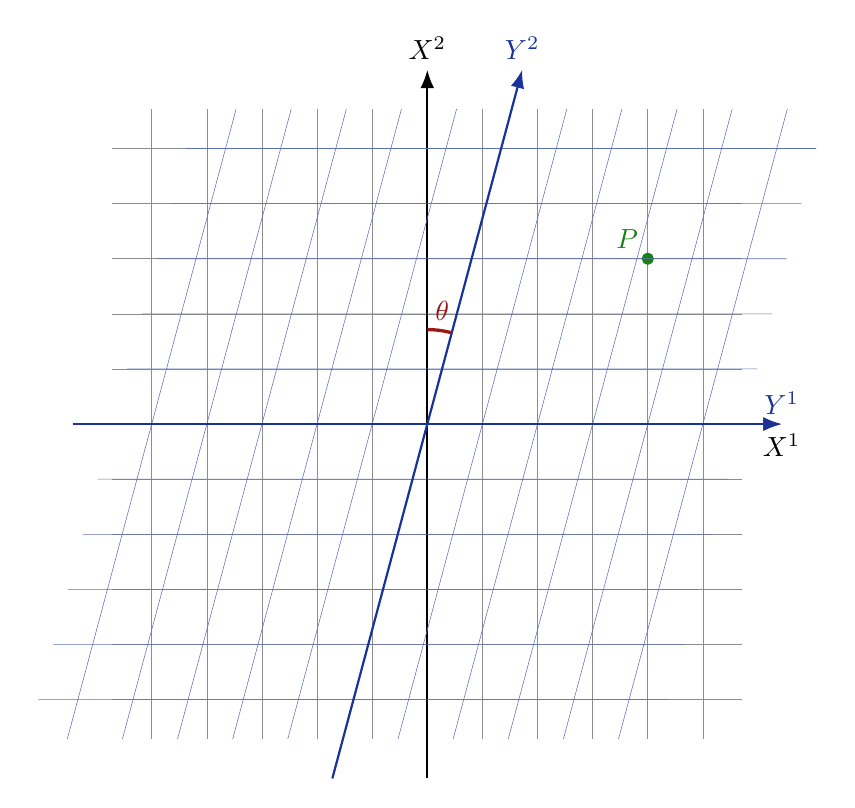
\begin{tikzpicture}
    \tikzstyle{axis_style} = [-Latex, thick, black]
    \tikzstyle{y_axis_style} = [-Latex, thick, darkblue]

    \def\px{4*0.7}
    \def\py{3*0.7}
    \def\angle{15}
    
    \begin{scope}
      \draw[step=0.7cm, color=gray!90, very thin] (-4,-4) grid (4,4);
      \draw[axis_style] (-4.5,0) -- (4.5,0);
      \draw[axis_style] (0,-4.5) -- (0,4.5) node[above] {$X^2$};
      \filldraw[darkgreen] (\px,\py) circle (2pt) node[above left] {$P$};
  	\end{scope}
    
    \begin{scope} [xslant=tan(15)]
      \draw[step=0.7cm, color=darkblue!70, very thin] (-4,-4) grid (4,4);
      \draw[y_axis_style] (-4.5,0) -- (4.5,0);
	    \draw[y_axis_style] (0,-4.5) -- (0,4.5) node[above] {$Y^2$};
    \end{scope}

    \node[below] at (4.5, 0) {$X^1$};
    \node[above, color=darkblue] at (4.5, 0) {$Y^1$};

    \coordinate (O) at (0,0);
    \coordinate (A) at (0, 2);
    \coordinate (B) at ({2*tan(\angle)}, 2);
    
    \pic [draw=darkred, very thick, angle radius=1.2cm] {angle = B--O--A};
    \node[darkred] at (90-\angle/2:1.45cm) {$\theta$};
\end{tikzpicture}
\end{document}
